% REV01 Tue 22 Jun 2021 17:46:08 WIB
% START Tue 04 May 2021 13:55:16 WIB

\chapter{MERCURY PROMPTING}

Fledgeby deserved Mr Alfred Lammle’s eulogium. He was the meanest
cur existing, with a single pair of legs. And instinct (a word we all
clearly understand) going largely on four legs, and reason always on
two, meanness on four legs never attains the perfection of meanness on
two.

The father of this young gentleman had been a money-lender, who
had transacted professional business with the mother of this
young gentleman, when he, the latter, was waiting in the vast dark
ante-chambers of the present world to be born. The lady, a widow, being
unable to pay the money-lender, married him; and in due course, Fledgeby
was summoned out of the vast dark ante-chambers to come and be presented
to the Registrar-General. Rather a curious speculation how Fledgeby
would otherwise have disposed of his leisure until Doomsday.

Fledgeby’s mother offended her family by marrying Fledgeby’s father. It
is one of the easiest achievements in life to offend your family when
your family want to get rid of you. Fledgeby’s mother’s family had
been very much offended with her for being poor, and broke with her
for becoming comparatively rich. Fledgeby’s mother’s family was the
Snigsworth family. She had even the high honour to be cousin to Lord
Snigsworth--so many times removed that the noble Earl would have had no
compunction in removing her one time more and dropping her clean outside
the cousinly pale; but cousin for all that.

Among her pre-matrimonial transactions with Fledgeby’s father,
Fledgeby’s mother had raised money of him at a great disadvantage on a
certain reversionary interest. The reversion falling in soon after they
were married, Fledgeby’s father laid hold of the cash for his separate
use and benefit. This led to subjective differences of opinion, not to
say objective interchanges of boot-jacks, backgammon boards, and other
such domestic missiles, between Fledgeby’s father and Fledgeby’s mother,
and those led to Fledgeby’s mother spending as much money as she
could, and to Fledgeby’s father doing all he couldn’t to restrain her.
Fledgeby’s childhood had been, in consequence, a stormy one; but the
winds and the waves had gone down in the grave, and Fledgeby flourished
alone.

He lived in chambers in the Albany, did Fledgeby, and maintained a
spruce appearance. But his youthful fire was all composed of sparks from
the grindstone; and as the sparks flew off, went out, and never warmed
anything, be sure that Fledgeby had his tools at the grindstone, and
turned it with a wary eye.

Mr Alfred Lammle came round to the Albany to breakfast with Fledgeby.
Present on the table, one scanty pot of tea, one scanty loaf, two scanty
pats of butter, two scanty rashers of bacon, two pitiful eggs, and an
abundance of handsome china bought a secondhand bargain.

‘What did you think of Georgiana?’ asked Mr Lammle.

‘Why, I’ll tell you,’ said Fledgeby, very deliberately.

‘Do, my boy.’

‘You misunderstand me,’ said Fledgeby. ‘I don’t mean I’ll tell you that.
I mean I’ll tell you something else.’

‘Tell me anything, old fellow!’

‘Ah, but there you misunderstand me again,’ said Fledgeby. ‘I mean I’ll
tell you nothing.’

Mr Lammle sparkled at him, but frowned at him too.

‘Look here,’ said Fledgeby. ‘You’re deep and you’re ready. Whether I am
deep or not, never mind. I am not ready. But I can do one thing, Lammle,
I can hold my tongue. And I intend always doing it.’

‘You are a long-headed fellow, Fledgeby.’

‘May be, or may not be. If I am a short-tongued fellow, it may amount to
the same thing. Now, Lammle, I am never going to answer questions.’

‘My dear fellow, it was the simplest question in the world.’

‘Never mind. It seemed so, but things are not always what they seem. I
saw a man examined as a witness in Westminster Hall. Questions put to
him seemed the simplest in the world, but turned out to be anything
rather than that, after he had answered ‘em. Very well. Then he should
have held his tongue. If he had held his tongue he would have kept out
of scrapes that he got into.’

‘If I had held my tongue, you would never have seen the subject of my
question,’ remarked Lammle, darkening.

‘Now, Lammle,’ said Fascination Fledgeby, calmly feeling for his
whisker, ‘it won’t do. I won’t be led on into a discussion. I can’t
manage a discussion. But I can manage to hold my tongue.’

‘Can?’ Mr Lammle fell back upon propitiation. ‘I should think you could!
Why, when these fellows of our acquaintance drink and you drink with
them, the more talkative they get, the more silent you get. The more
they let out, the more you keep in.’

‘I don’t object, Lammle,’ returned Fledgeby, with an internal chuckle,
‘to being understood, though I object to being questioned. That
certainly IS the way I do it.’

‘And when all the rest of us are discussing our ventures, none of us
ever know what a single venture of yours is!’

‘And none of you ever will from me, Lammle,’ replied Fledgeby, with
another internal chuckle; ‘that certainly IS the way I do it.’

‘Why of course it is, I know!’ rejoined Lammle, with a flourish of
frankness, and a laugh, and stretching out his hands as if to show
the universe a remarkable man in Fledgeby. ‘If I hadn’t known it of my
Fledgeby, should I have proposed our little compact of advantage, to my
Fledgeby?’

‘Ah!’ remarked Fascination, shaking his head slyly. ‘But I am not to
be got at in that way. I am not vain. That sort of vanity don’t pay,
Lammle. No, no, no. Compliments only make me hold my tongue the more.’

Alfred Lammle pushed his plate away (no great sacrifice under the
circumstances of there being so little in it), thrust his hands in his
pockets, leaned back in his chair, and contemplated Fledgeby in silence.
Then he slowly released his left hand from its pocket, and made that
bush of his whiskers, still contemplating him in silence. Then he slowly
broke silence, and slowly said: ‘What--the--Dev-il is this fellow about
this morning?’

‘Now, look here, Lammle,’ said Fascination Fledgeby, with the meanest
of twinkles in his meanest of eyes: which were too near together, by
the way: ‘look here, Lammle; I am very well aware that I didn’t show to
advantage last night, and that you and your wife--who, I consider, is
a very clever woman and an agreeable woman--did. I am not calculated to
show to advantage under that sort of circumstances. I know very well you
two did show to advantage, and managed capitally. But don’t you on that
account come talking to me as if I was your doll and puppet, because I
am not.

‘And all this,’ cried Alfred, after studying with a look the meanness
that was fain to have the meanest help, and yet was so mean as to turn
upon it: ‘all this because of one simple natural question!’

‘You should have waited till I thought proper to say something about it
of myself. I don’t like your coming over me with your Georgianas, as if
you was her proprietor and mine too.’

‘Well, when you are in the gracious mind to say anything about it of
yourself,’ retorted Lammle, ‘pray do.’

‘I have done it. I have said you managed capitally. You and your wife
both. If you’ll go on managing capitally, I’ll go on doing my part. Only
don’t crow.’

‘I crow!’ exclaimed Lammle, shrugging his shoulders.

‘Or,’ pursued the other--‘or take it in your head that people are your
puppets because they don’t come out to advantage at the particular
moments when you do, with the assistance of a very clever and agreeable
wife. All the rest keep on doing, and let Mrs Lammle keep on doing. Now,
I have held my tongue when I thought proper, and I have spoken when I
thought proper, and there’s an end of that. And now the question is,’
proceeded Fledgeby, with the greatest reluctance, ‘will you have another
egg?’

‘No, I won’t,’ said Lammle, shortly.

‘Perhaps you’re right and will find yourself better without it,’ replied
Fascination, in greatly improved spirits. ‘To ask you if you’ll have
another rasher would be unmeaning flattery, for it would make you
thirsty all day. Will you have some more bread and butter?’

‘No, I won’t,’ repeated Lammle.

‘Then I will,’ said Fascination. And it was not a mere retort for the
sound’s sake, but was a cheerful cogent consequence of the refusal; for
if Lammle had applied himself again to the loaf, it would have been so
heavily visited, in Fledgeby’s opinion, as to demand abstinence from
bread, on his part, for the remainder of that meal at least, if not for
the whole of the next.

Whether this young gentleman (for he was but three-and-twenty) combined
with the miserly vice of an old man, any of the open-handed vices of
a young one, was a moot point; so very honourably did he keep his own
counsel. He was sensible of the value of appearances as an investment,
and liked to dress well; but he drove a bargain for every moveable about
him, from the coat on his back to the china on his breakfast-table;
and every bargain by representing somebody’s ruin or somebody’s loss,
acquired a peculiar charm for him. It was a part of his avarice to take,
within narrow bounds, long odds at races; if he won, he drove harder
bargains; if he lost, he half starved himself until next time. Why money
should be so precious to an Ass too dull and mean to exchange it for any
other satisfaction, is strange; but there is no animal so sure to get
laden with it, as the Ass who sees nothing written on the face of the
earth and sky but the three letters L. S. D.--not Luxury, Sensuality,
Dissoluteness, which they often stand for, but the three dry letters.
Your concentrated Fox is seldom comparable to your concentrated Ass in
money-breeding.

Fascination Fledgeby feigned to be a young gentleman living on his
means, but was known secretly to be a kind of outlaw in the bill-broking
line, and to put money out at high interest in various ways. His circle
of familiar acquaintance, from Mr Lammle round, all had a touch of the
outlaw, as to their rovings in the merry greenwood of Jobbery Forest,
lying on the outskirts of the Share-Market and the Stock Exchange.

‘I suppose you, Lammle,’ said Fledgeby, eating his bread and butter,
‘always did go in for female society?’

‘Always,’ replied Lammle, glooming considerably under his late
treatment.

‘Came natural to you, eh?’ said Fledgeby.

‘The sex were pleased to like me, sir,’ said Lammle sulkily, but with
the air of a man who had not been able to help himself.

‘Made a pretty good thing of marrying, didn’t you?’ asked Fledgeby.

The other smiled (an ugly smile), and tapped one tap upon his nose.

‘My late governor made a mess of it,’ said Fledgeby. ‘But Geor--is the
right name Georgina or Georgiana?’

‘Georgiana.’

‘I was thinking yesterday, I didn’t know there was such a name. I
thought it must end in ina.’

‘Why?’

‘Why, you play--if you can--the Concertina, you know,’ replied
Fledgeby, meditating very slowly. ‘And you have--when you catch it--the
Scarlatina. And you can come down from a balloon in a parach--no you
can’t though. Well, say Georgeute--I mean Georgiana.’

‘You were going to remark of Georgiana--?’ Lammle moodily hinted, after
waiting in vain.

‘I was going to remark of Georgiana, sir,’ said Fledgeby, not at all
pleased to be reminded of his having forgotten it, ‘that she don’t seem
to be violent. Don’t seem to be of the pitching-in order.’

‘She has the gentleness of the dove, Mr Fledgeby.’

‘Of course you’ll say so,’ replied Fledgeby, sharpening, the moment his
interest was touched by another. ‘But you know, the real look-out is
this:--what I say, not what you say. I say having my late governor
and my late mother in my eye--that Georgiana don’t seem to be of the
pitching-in order.’

The respected Mr Lammle was a bully, by nature and by usual practice.
Perceiving, as Fledgeby’s affronts cumulated, that conciliation by no
means answered the purpose here, he now directed a scowling look
into Fledgeby’s small eyes for the effect of the opposite treatment.
Satisfied by what he saw there, he burst into a violent passion and
struck his hand upon the table, making the china ring and dance.

‘You are a very offensive fellow, sir,’ cried Mr Lammle, rising. ‘You
are a highly offensive scoundrel. What do you mean by this behaviour?’

‘I say!’ remonstrated Fledgeby. ‘Don’t break out.’

‘You are a very offensive fellow sir,’ repeated Mr Lammle. ‘You are a
highly offensive scoundrel!’

‘I SAY, you know!’ urged Fledgeby, quailing.

‘Why, you coarse and vulgar vagabond!’ said Mr Lammle, looking fiercely
about him, ‘if your servant was here to give me sixpence of your
money to get my boots cleaned afterwards--for you are not worth the
expenditure--I’d kick you.’

‘No you wouldn’t,’ pleaded Fledgeby. ‘I am sure you’d think better of
it.’

‘I tell you what, Mr Fledgeby,’ said Lammle advancing on him. ‘Since
you presume to contradict me, I’ll assert myself a little. Give me your
nose!’

Fledgeby covered it with his hand instead, and said, retreating, ‘I beg
you won’t!’

‘Give me your nose, sir,’ repeated Lammle.

Still covering that feature and backing, Mr Fledgeby reiterated
(apparently with a severe cold in his head), ‘I beg, I beg, you won’t.’

‘And this fellow,’ exclaimed Lammle, stopping and making the most of his
chest--‘This fellow presumes on my having selected him out of all the
young fellows I know, for an advantageous opportunity! This fellow
presumes on my having in my desk round the corner, his dirty note of
hand for a wretched sum payable on the occurrence of a certain event,
which event can only be of my and my wife’s bringing about! This fellow,
Fledgeby, presumes to be impertinent to me, Lammle. Give me your nose
sir!’

‘No! Stop! I beg your pardon,’ said Fledgeby, with humility.

‘What do you say, sir?’ demanded Mr Lammle, seeming too furious to
understand.

‘I beg your pardon,’ repeated Fledgeby.

‘Repeat your words louder, sir. The just indignation of a gentleman has
sent the blood boiling to my head. I don’t hear you.’

‘I say,’ repeated Fledgeby, with laborious explanatory politeness, ‘I
beg your pardon.’

Mr Lammle paused. ‘As a man of honour,’ said he, throwing himself into a
chair, ‘I am disarmed.’

Mr Fledgeby also took a chair, though less demonstratively, and by
slow approaches removed his hand from his nose. Some natural diffidence
assailed him as to blowing it, so shortly after its having assumed a
personal and delicate, not to say public, character; but he overcame
his scruples by degrees, and modestly took that liberty under an implied
protest.

‘Lammle,’ he said sneakingly, when that was done, ‘I hope we are friends
again?’

‘Mr Fledgeby,’ returned Lammle, ‘say no more.’

‘I must have gone too far in making myself disagreeable,’ said Fledgeby,
‘but I never intended it.’

‘Say no more, say no more!’ Mr Lammle repeated in a magnificent tone.
‘Give me your’--Fledgeby started--‘hand.’

They shook hands, and on Mr Lammle’s part, in particular, there ensued
great geniality. For, he was quite as much of a dastard as the other,
and had been in equal danger of falling into the second place for good,
when he took heart just in time, to act upon the information conveyed to
him by Fledgeby’s eye.

The breakfast ended in a perfect understanding. Incessant machinations
were to be kept at work by Mr and Mrs Lammle; love was to be made for
Fledgeby, and conquest was to be insured to him; he on his part
very humbly admitting his defects as to the softer social arts, and
entreating to be backed to the utmost by his two able coadjutors.

Little recked Mr Podsnap of the traps and toils besetting his Young
Person. He regarded her as safe within the Temple of Podsnappery, hiding
the fulness of time when she, Georgiana, should take him, Fitz-Podsnap,
who with all his worldly goods should her endow. It would call a blush
into the cheek of his standard Young Person to have anything to do with
such matters save to take as directed, and with worldly goods as per
settlement to be endowed. Who giveth this woman to be married to this
man? I, Podsnap. Perish the daring thought that any smaller creation
should come between!

It was a public holiday, and Fledgeby did not recover his spirits or his
usual temperature of nose until the afternoon. Walking into the City in
the holiday afternoon, he walked against a living stream setting out of
it; and thus, when he turned into the precincts of St Mary Axe, he found
a prevalent repose and quiet there. A yellow overhanging plaster-fronted
house at which he stopped was quiet too. The blinds were all drawn down,
and the inscription Pubsey and Co. seemed to doze in the counting-house
window on the ground-floor giving on the sleepy street.

Fledgeby knocked and rang, and Fledgeby rang and knocked, but no
one came. Fledgeby crossed the narrow street and looked up at the
house-windows, but nobody looked down at Fledgeby. He got out of temper,
crossed the narrow street again, and pulled the housebell as if it were
the house’s nose, and he were taking a hint from his late experience.
His ear at the keyhole seemed then, at last, to give him assurance that
something stirred within. His eye at the keyhole seemed to confirm his
ear, for he angrily pulled the house’s nose again, and pulled and pulled
and continued to pull, until a human nose appeared in the dark doorway.

‘Now you sir!’ cried Fledgeby. ‘These are nice games!’

He addressed an old Jewish man in an ancient coat, long of skirt, and
wide of pocket. A venerable man, bald and shining at the top of his
head, and with long grey hair flowing down at its sides and mingling
with his beard. A man who with a graceful Eastern action of homage bent
his head, and stretched out his hands with the palms downward, as if to
deprecate the wrath of a superior.

‘What have you been up to?’ said Fledgeby, storming at him.

‘Generous Christian master,’ urged the Jewish man, ‘it being holiday, I
looked for no one.’

‘Holiday he blowed!’ said Fledgeby, entering. ‘What have YOU got to do
with holidays? Shut the door.’

With his former action the old man obeyed. In the entry hung his rusty
large-brimmed low-crowned hat, as long out of date as his coat; in the
corner near it stood his staff--no walking-stick but a veritable staff.
Fledgeby turned into the counting-house, perched himself on a business
stool, and cocked his hat. There were light boxes on shelves in the
counting-house, and strings of mock beads hanging up. There were samples
of cheap clocks, and samples of cheap vases of flowers. Foreign toys,
all.

Perched on the stool with his hat cocked on his head and one of his legs
dangling, the youth of Fledgeby hardly contrasted to advantage with the
age of the Jewish man as he stood with his bare head bowed, and his eyes
(which he only raised in speaking) on the ground. His clothing was worn
down to the rusty hue of the hat in the entry, but though he looked
shabby he did not look mean. Now, Fledgeby, though not shabby, did look
mean.

‘You have not told me what you were up to, you sir,’ said Fledgeby,
scratching his head with the brim of his hat.

‘Sir, I was breathing the air.’

‘In the cellar, that you didn’t hear?’

‘On the house-top.’

‘Upon my soul! That’s a way of doing business.’

‘Sir,’ the old man represented with a grave and patient air, ‘there must
be two parties to the transaction of business, and the holiday has left
me alone.’

‘Ah! Can’t be buyer and seller too. That’s what the Jews say; ain’t it?’

‘At least we say truly, if we say so,’ answered the old man with a
smile.

‘Your people need speak the truth sometimes, for they lie enough,’
remarked Fascination Fledgeby.

‘Sir, there is,’ returned the old man with quiet emphasis, ‘too much
untruth among all denominations of men.’

Rather dashed, Fascination Fledgeby took another scratch at his
intellectual head with his hat, to gain time for rallying.

‘For instance,’ he resumed, as though it were he who had spoken last,
‘who but you and I ever heard of a poor Jew?’

‘The Jews,’ said the old man, raising his eyes from the ground with his
former smile. ‘They hear of poor Jews often, and are very good to them.’

‘Bother that!’ returned Fledgeby. ‘You know what I mean. You’d persuade
me if you could, that you are a poor Jew. I wish you’d confess how much
you really did make out of my late governor. I should have a better
opinion of you.’

The old man only bent his head, and stretched out his hands as before.

‘Don’t go on posturing like a Deaf and Dumb School,’ said the ingenious
Fledgeby, ‘but express yourself like a Christian--or as nearly as you
can.’

‘I had had sickness and misfortunes, and was so poor,’ said the old
man, ‘as hopelessly to owe the father, principal and interest. The son
inheriting, was so merciful as to forgive me both, and place me here.’

He made a little gesture as though he kissed the hem of an imaginary
garment worn by the noble youth before him. It was humbly done, but
picturesquely, and was not abasing to the doer.

‘You won’t say more, I see,’ said Fledgeby, looking at him as if he
would like to try the effect of extracting a double-tooth or two, ‘and
so it’s of no use my putting it to you. But confess this, Riah; who
believes you to be poor now?’

‘No one,’ said the old man.

‘There you’re right,’ assented Fledgeby.

‘No one,’ repeated the old man with a grave slow wave of his head. ‘All
scout it as a fable. Were I to say “This little fancy business is not
mine”;’ with a lithe sweep of his easily-turning hand around him,
to comprehend the various objects on the shelves; ‘“it is the little
business of a Christian young gentleman who places me, his servant, in
trust and charge here, and to whom I am accountable for every single
bead,” they would laugh. When, in the larger money-business, I tell the
borrowers--’

‘I say, old chap!’ interposed Fledgeby, ‘I hope you mind what you DO
tell ‘em?’

‘Sir, I tell them no more than I am about to repeat. When I tell them,
“I cannot promise this, I cannot answer for the other, I must see my
principal, I have not the money, I am a poor man and it does not rest
with me,” they are so unbelieving and so impatient, that they sometimes
curse me in Jehovah’s name.’

‘That’s deuced good, that is!’ said Fascination Fledgeby.

‘And at other times they say, “Can it never be done without these
tricks, Mr Riah? Come, come, Mr Riah, we know the arts of your
people”--my people!--“If the money is to be lent, fetch it, fetch it; if
it is not to be lent, keep it and say so.” They never believe me.’

‘THAT’S all right,’ said Fascination Fledgeby.

‘They say, “We know, Mr Riah, we know. We have but to look at you, and
we know.”’

‘Oh, a good ‘un are you for the post,’ thought Fledgeby, ‘and a good ‘un
was I to mark you out for it! I may be slow, but I am precious sure.’

Not a syllable of this reflection shaped itself in any scrap of Mr
Fledgeby’s breath, lest it should tend to put his servant’s price up.
But looking at the old man as he stood quiet with his head bowed and his
eyes cast down, he felt that to relinquish an inch of his baldness,
an inch of his grey hair, an inch of his coat-skirt, an inch of his
hat-brim, an inch of his walking-staff, would be to relinquish hundreds
of pounds.

‘Look here, Riah,’ said Fledgeby, mollified by these self-approving
considerations. ‘I want to go a little more into buying-up queer bills.
Look out in that direction.’

‘Sir, it shall be done.’

‘Casting my eye over the accounts, I find that branch of business pays
pretty fairly, and I am game for extending it. I like to know people’s
affairs likewise. So look out.’

‘Sir, I will, promptly.’

‘Put it about in the right quarters, that you’ll buy queer bills by the
lump--by the pound weight if that’s all--supposing you see your way to a
fair chance on looking over the parcel. And there’s one thing more. Come
to me with the books for periodical inspection as usual, at eight on
Monday morning.’

Riah drew some folding tablets from his breast and noted it down.

‘That’s all I wanted to say at the present time,’ continued Fledgeby in
a grudging vein, as he got off the stool, ‘except that I wish you’d take
the air where you can hear the bell, or the knocker, either one of the
two or both. By-the-by how DO you take the air at the top of the house?
Do you stick your head out of a chimney-pot?’

‘Sir, there are leads there, and I have made a little garden there.’

‘To bury your money in, you old dodger?’

‘A thumbnail’s space of garden would hold the treasure I bury, master,’
said Riah. ‘Twelve shillings a week, even when they are an old man’s
wages, bury themselves.’

‘I should like to know what you really are worth,’ returned Fledgeby,
with whom his growing rich on that stipend and gratitude was a very
convenient fiction. ‘But come! Let’s have a look at your garden on the
tiles, before I go!’

The old man took a step back, and hesitated.

‘Truly, sir, I have company there.’

‘Have you, by George!’ said Fledgeby; ‘I suppose you happen to know
whose premises these are?’

‘Sir, they are yours, and I am your servant in them.’

‘Oh! I thought you might have overlooked that,’ retorted Fledgeby, with
his eyes on Riah’s beard as he felt for his own; ‘having company on my
premises, you know!’

‘Come up and see the guests, sir. I hope for your admission that they
can do no harm.’

Passing him with a courteous reverence, specially unlike any action that
Mr Fledgeby could for his life have imparted to his own head and hands,
the old man began to ascend the stairs. As he toiled on before, with his
palm upon the stair-rail, and his long black skirt, a very gaberdine,
overhanging each successive step, he might have been the leader in some
pilgrimage of devotional ascent to a prophet’s tomb. Not troubled by any
such weak imagining, Fascination Fledgeby merely speculated on the time
of life at which his beard had begun, and thought once more what a good
‘un he was for the part.

Some final wooden steps conducted them, stooping under a low penthouse
roof, to the house-top. Riah stood still, and, turning to his master,
pointed out his guests.

Lizzie Hexam and Jenny Wren. For whom, perhaps with some old instinct of
his race, the gentle Jew had spread a carpet. Seated on it, against
no more romantic object than a blackened chimney-stack over which some
bumble creeper had been trained, they both pored over one book; both
with attentive faces; Jenny with the sharper; Lizzie with the more
perplexed. Another little book or two were lying near, and a common
basket of common fruit, and another basket full of strings of beads and
tinsel scraps. A few boxes of humble flowers and evergreens completed
the garden; and the encompassing wilderness of dowager old chimneys
twirled their cowls and fluttered their smoke, rather as if they were
bridling, and fanning themselves, and looking on in a state of airy
surprise.

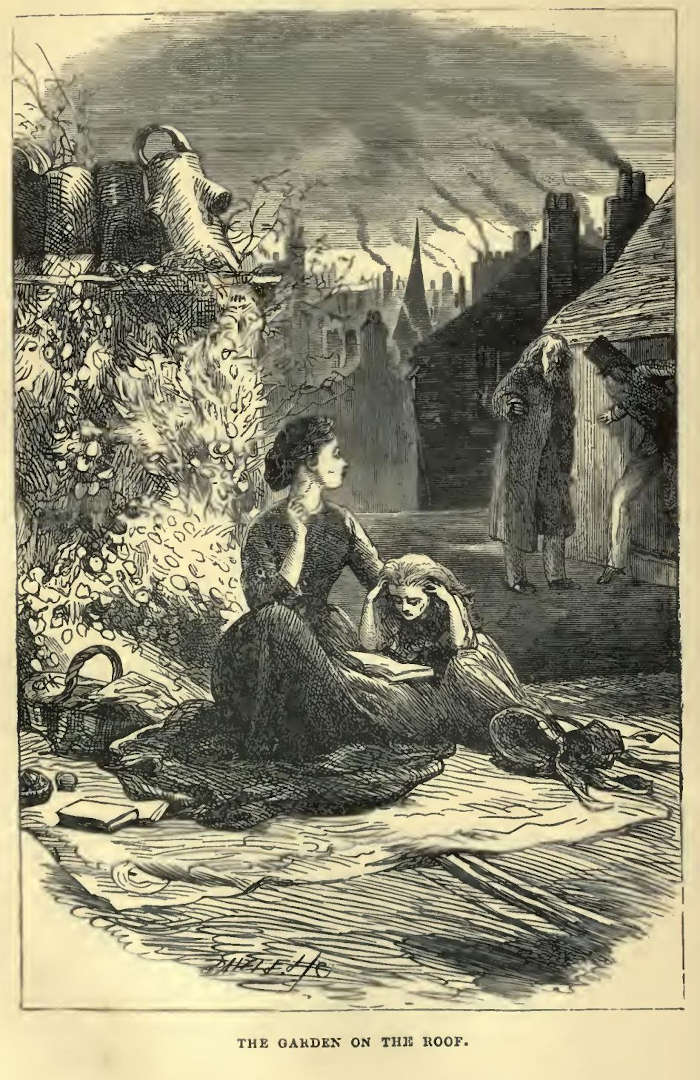
\includegraphics[scale=2.3]{02-05-01}

Taking her eyes off the book, to test her memory of something in it,
Lizzie was the first to see herself observed. As she rose, Miss Wren
likewise became conscious, and said, irreverently addressing the great
chief of the premises: ‘Whoever you are, I can’t get up, because my
back’s bad and my legs are queer.’

‘This is my master,’ said Riah, stepping forward.

(‘Don’t look like anybody’s master,’ observed Miss Wren to herself, with
a hitch of her chin and eyes.)

‘This, sir,’ pursued the old man, ‘is a little dressmaker for little
people. Explain to the master, Jenny.’

‘Dolls; that’s all,’ said Jenny, shortly. ‘Very difficult to fit too,
because their figures are so uncertain. You never know where to expect
their waists.’

‘Her friend,’ resumed the old man, motioning towards Lizzie; ‘and as
industrious as virtuous. But that they both are. They are busy early and
late, sir, early and late; and in bye-times, as on this holiday, they go
to book-learning.’

‘Not much good to be got out of that,’ remarked Fledgeby.

‘Depends upon the person!’ quoth Miss Wren, snapping him up.

‘I made acquaintance with my guests, sir,’ pursued the Jew, with an
evident purpose of drawing out the dressmaker, ‘through their coming
here to buy of our damage and waste for Miss Jenny’s millinery. Our
waste goes into the best of company, sir, on her rosy-cheeked little
customers. They wear it in their hair, and on their ball-dresses, and
even (so she tells me) are presented at Court with it.’

‘Ah!’ said Fledgeby, on whose intelligence this doll-fancy made rather
strong demands; ‘she’s been buying that basketful to-day, I suppose?’

‘I suppose she has,’ Miss Jenny interposed; ‘and paying for it too, most
likely!’

‘Let’s have a look at it,’ said the suspicious chief. Riah handed it to
him. ‘How much for this now?’

‘Two precious silver shillings,’ said Miss Wren.

Riah confirmed her with two nods, as Fledgeby looked to him. A nod for
each shilling.

‘Well,’ said Fledgeby, poking into the contents of the basket with his
forefinger, ‘the price is not so bad. You have got good measure, Miss
What-is-it.’

‘Try Jenny,’ suggested that young lady with great calmness.

‘You have got good measure, Miss Jenny; but the price is not so
bad.--And you,’ said Fledgeby, turning to the other visitor, ‘do you buy
anything here, miss?’

‘No, sir.’

‘Nor sell anything neither, miss?’

‘No, sir.’

Looking askew at the questioner, Jenny stole her hand up to her
friend’s, and drew her friend down, so that she bent beside her on her
knee.

‘We are thankful to come here for rest, sir,’ said Jenny. ‘You see, you
don’t know what the rest of this place is to us; does he, Lizzie? It’s
the quiet, and the air.’

‘The quiet!’ repeated Fledgeby, with a contemptuous turn of his head
towards the City’s roar. ‘And the air!’ with a ‘Poof!’ at the smoke.

‘Ah!’ said Jenny. ‘But it’s so high. And you see the clouds rushing
on above the narrow streets, not minding them, and you see the golden
arrows pointing at the mountains in the sky from which the wind comes,
and you feel as if you were dead.’

The little creature looked above her, holding up her slight transparent
hand.

‘How do you feel when you are dead?’ asked Fledgeby, much perplexed.

‘Oh, so tranquil!’ cried the little creature, smiling. ‘Oh, so peaceful
and so thankful! And you hear the people who are alive, crying, and
working, and calling to one another down in the close dark streets, and
you seem to pity them so! And such a chain has fallen from you, and such
a strange good sorrowful happiness comes upon you!’

Her eyes fell on the old man, who, with his hands folded, quietly looked
on.

‘Why it was only just now,’ said the little creature, pointing at him,
‘that I fancied I saw him come out of his grave! He toiled out at
that low door so bent and worn, and then he took his breath and stood
upright, and looked all round him at the sky, and the wind blew upon
him, and his life down in the dark was over!--Till he was called back
to life,’ she added, looking round at Fledgeby with that lower look of
sharpness. ‘Why did you call him back?’

‘He was long enough coming, anyhow,’ grumbled Fledgeby.

‘But you are not dead, you know,’ said Jenny Wren. ‘Get down to life!’

Mr Fledgeby seemed to think it rather a good suggestion, and with a nod
turned round. As Riah followed to attend him down the stairs, the little
creature called out to the Jew in a silvery tone, ‘Don’t be long gone.
Come back, and be dead!’ And still as they went down they heard the
little sweet voice, more and more faintly, half calling and half
singing, ‘Come back and be dead, Come back and be dead!’

When they got down into the entry, Fledgeby, pausing under the shadow of
the broad old hat, and mechanically poising the staff, said to the old
man:

‘That’s a handsome girl, that one in her senses.’

‘And as good as handsome,’ answered Riah.

‘At all events,’ observed Fledgeby, with a dry whistle, ‘I hope she
ain’t bad enough to put any chap up to the fastenings, and get the
premises broken open. You look out. Keep your weather eye awake and
don’t make any more acquaintances, however handsome. Of course you
always keep my name to yourself?’

‘Sir, assuredly I do.’

‘If they ask it, say it’s Pubsey, or say it’s Co, or say it’s anything
you like, but what it is.’

His grateful servant--in whose race gratitude is deep, strong, and
enduring--bowed his head, and actually did now put the hem of his coat
to his lips: though so lightly that the wearer knew nothing of it.

Thus, Fascination Fledgeby went his way, exulting in the artful
cleverness with which he had turned his thumb down on a Jew, and the old
man went his different way up-stairs. As he mounted, the call or song
began to sound in his ears again, and, looking above, he saw the face
of the little creature looking down out of a Glory of her long bright
radiant hair, and musically repeating to him, like a vision:

‘Come up and be dead! Come up and be dead!’



